%%
%% Author: Dario Chinelli
%% begin 2019-12-04
%% last mod 2022-02-02
%%

% Preamble
\documentclass[class=article, crop=false]{standalone}

% Packages
\usepackage[subpreambles=true]{standalone}
\usepackage{import}
\usepackage{graphicx}
\usepackage{amsmath}
\usepackage{subfig}

%	References:
%	> Markov chains  from theory to implementation and experimentation by Gagniuc, Paul A

% Document
\begin{document}\label{chap:MarkovChain}

A \emph{Markov Chain} (MC) is a stochastic model. 
It predicts the future outcoming state based on the present one. 
In other words, the present state determinates the probabilities for every possible future outcome. 
The MC may be represented as a diagram (Figure \ref{fig:diagramMC}) \cite{MC_Gagniuc} in which the arrows are the possible transitions. 
A number $p \in (0,1)$ may also be indicated on the arrows to specifies the probability of that transition. 
Another model’s representation is a \emph{stochastic matrix}, also called $P$ matrix. 
The matrix entries $P_{ij}$ have as row-index i the starting state and as column-index j the ending state of the system. 
Hence, all the entries are referred to a specific transition. 
A two-state Markov Chain is the most basic model, which can be used for the illustration of the Markov process. 
The diagram in (Figure \ref{fig:MarkovMatrix}) represents the possibility that the system must change from both states. 
For instance, from the state $W$ the system can move to the state $B$ with the big black arrow or can remain in the state $W$ with the small white arrow.
The entries in the Markov Matrix in (Figure \ref{fig:matrixMC}) are positives numbers from $0$ to $1$; they represent the probability of changing state. 
The sum on the outgoing arrows must be equal to $1$.

\begin{figure}[h]
    \centering
    \subfloat[The diagram of a two-state Markov Chain]{
    \label{fig:diagramMC}
        
\includegraphics[ width=0.32\textwidth]{./estratti/Markov Chain scheme two state}
    }\quad\quad
    \subfloat[The transition matrix, also named the Markov matrix]{
    \label{fig:matrixMC}
        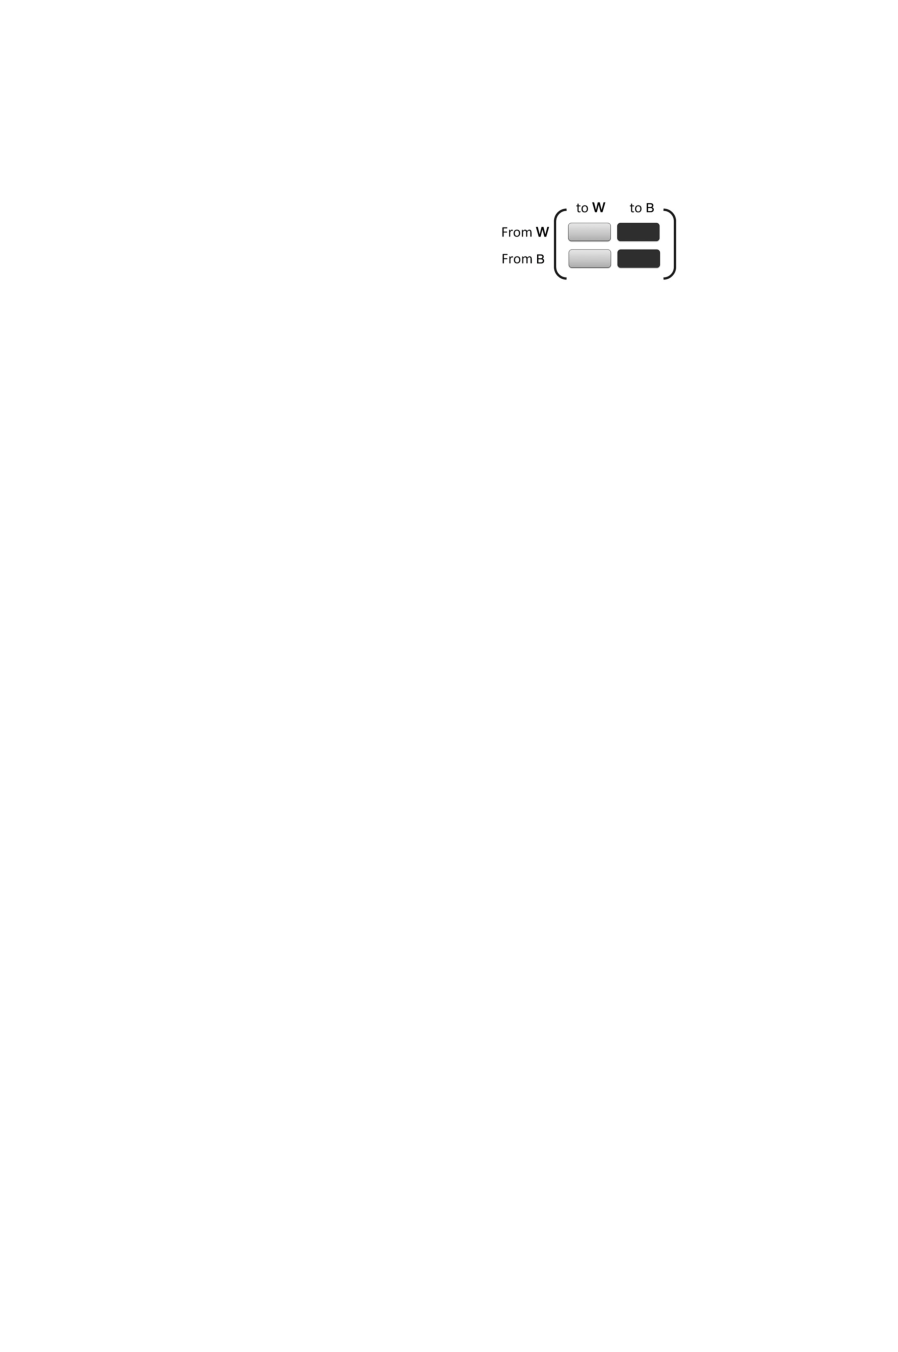
\includegraphics[ width=0.4\textwidth]{./estratti/Markov Chain matrix two state}
    }
    \caption{From the Markov diagram to the Markov matrix of a tow-state system.}
    \label{fig:MarkovMatrix}
\end{figure}





\end{document}
